\section{Datenbank}
- Daten in Verbindung setzen, keine redundanz
- Ordnung der Daten
- zentrale Speicherort
- Atomare Operation -> keine unvollständigen Daten
- Daten müssen erhalten bleiben
- Abfragen besser optimiert als auf Dateien
- Views zur Berechnung von Punkten

Daten haben Schema, Keine großen Datenmengen

-> relationale db

\subsection{ASDF-Tabellen}
\begin{center}
	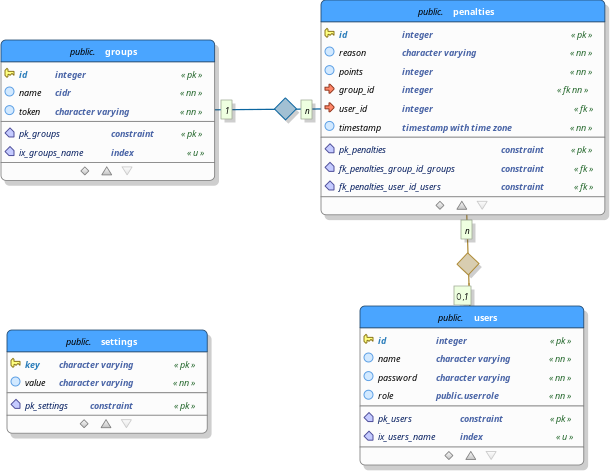
\includegraphics[width=\linewidth, keepaspectratio]{entwurf/datenbank/asdf-tabellen}
	\captionof{figure}{Ansicht der ASDF-Tabellen (ER-Diagramm)}
	\label{fig:db-asdf-table}
\end{center}

In der Abbildung \ref{fig:db-asdf-table} ist neben der alleinstehenden Tabelle \textbf{\textit{settings}} die Tabelle \textbf{\textit{users}} sowie die n zu m Beziehung zwischen \textbf{\textit{users}} und \textbf{\textit{groups}} dargestellt. Die n zum m Beziehung wird über eine Referenztabelle (\textbf{\textit{penalties}}) mit einer 1 zu n Beziehung zwischen \textbf{\textit{groups}} und \textbf{\textit{penalties}} und einer 0,1 zu n Beziehung zwischen \textbf{\textit{users}} und \textbf{\textit{penalties}} modelliert. In der n zu m Beziehung werden die ausgesprochen Strafen gespeichert. Jede Gruppe kann von mehreren Betreuern oder dem System mehrmals verwarnt werden.

\subsubsection{Einstellungen}
Die \textbf{\textit{settings}} Tabelle beinhaltet Einstellungen des Spiels als key-value Paar. Hierbei sind beide Spalten strings und der key einzigartig. Zu den Einstellungen gehört beispeilsweise das Scan-Intervall, die Flags pro Team sowie das Ende der Discover- und Attackzeit.

\subsubsection{Nutzer}
In der Tabelle \textbf{\textit{users}} sind die Log-In Informationen der Administratoren, Betreuer und Spieler hinterlegt. Da der Login aus Nutzername und Passwort besteht, werden die Spalten \textit{name} und \textit{password} benötigt. Auch muss anhand des Nutzernamens eindeutig auf einen Account geschlossen werden, deshalb ist die Spalte \textit{name} als unique gekennzeichnet. Die Rolle des Nutzers wird mithilfe eines Enums (\textit{role}) (Liste von benannten Werten) definiert.

\subsubsection{Strafen}
Die durch das System oder die Betreuer verteilten Strafen werden in der Tabelle \textbf{\textit{penalties}} gespeichert. Dazu wird neben dem Grund der Strafe (\textit{reason}), der Zeitpunkt der Bestrafung (\textit{timestamp}) auch die Anzahl an Strafpunkten (\textit{points}) festgehalten. Damit Gruppen von einem Betreuer öfters bestraft werden können, ist der Primärschlüssel des Eintrages die ID der Strafe.

\subsection{Gruppen-Tabellen}
\begin{center}
	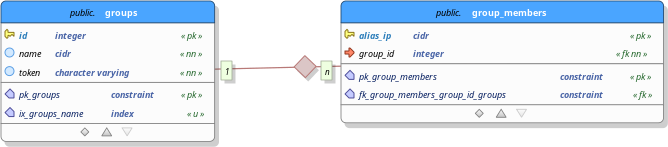
\includegraphics[width=\linewidth, keepaspectratio]{entwurf/datenbank/gruppen-tabellen}
	\captionof{figure}{Ansicht der Gruppen-Tabellen (ER-Diagramm)}
	\label{fig:db-group-table}
\end{center}

Wie in Abbildung \ref{fig:db-group-table} zusehen existiert zwischen der Tabelle \textbf{\textit{groups}} und \textbf{\textit{group\_members}} eine 1 zu n Beziehung. Dies bedeutete, dass eine Gruppe mehrere Mitglieder haben kann, aber jedes Mitglied nur genau in einer Gruppe vertreten sein kann.

\subsubsection{Gruppe}
In der Tabelle \textbf{\textit{groups}} werden alle teilnehmenden GameClients vermerkt. Jede Gruppe besitzt eine eindeutige \textit{ID} und einen eindeutigen \textit{Namen}. Der \textit{Name} der Gruppe repräsentiert die IP-Adresse des GameClients und ist nach Classless Internet Domain Routing Konvention (CIDR) abgelegt. Des Weiteren besitzt die \textbf{\textit{groups}} Tabelle die Spalte \textit{token}. In dieser wird der individuelle Token, welcher zur Flaggenerierung benötigt wird, abgespeichert. Dies ist nötig, damit der Server die selben Flags wie der GameClient generieren kann und die Betreuer die Richtigkeit verifizieren können.

\subsubsection{Gruppenmitglieder}
Die Tabelle \textbf{\textit{group\_members}} beinhaltet alle IP-Adressen, welche im Namen einer Gruppe agieren dürfen. Dafür wird die IP-Adresse im Feld \textit{alias\_ip} und die vertretende Gruppe als Referenz im Feld \textit{group\_id} gespeichert. Da das Feld \textit{alias\_ip} als Primärschlüssel verwendet wird, kann jede IP-Adresse nur genau eine Gruppe vertreten.

\subsection{Flags-Tabellen}
\begin{center}
	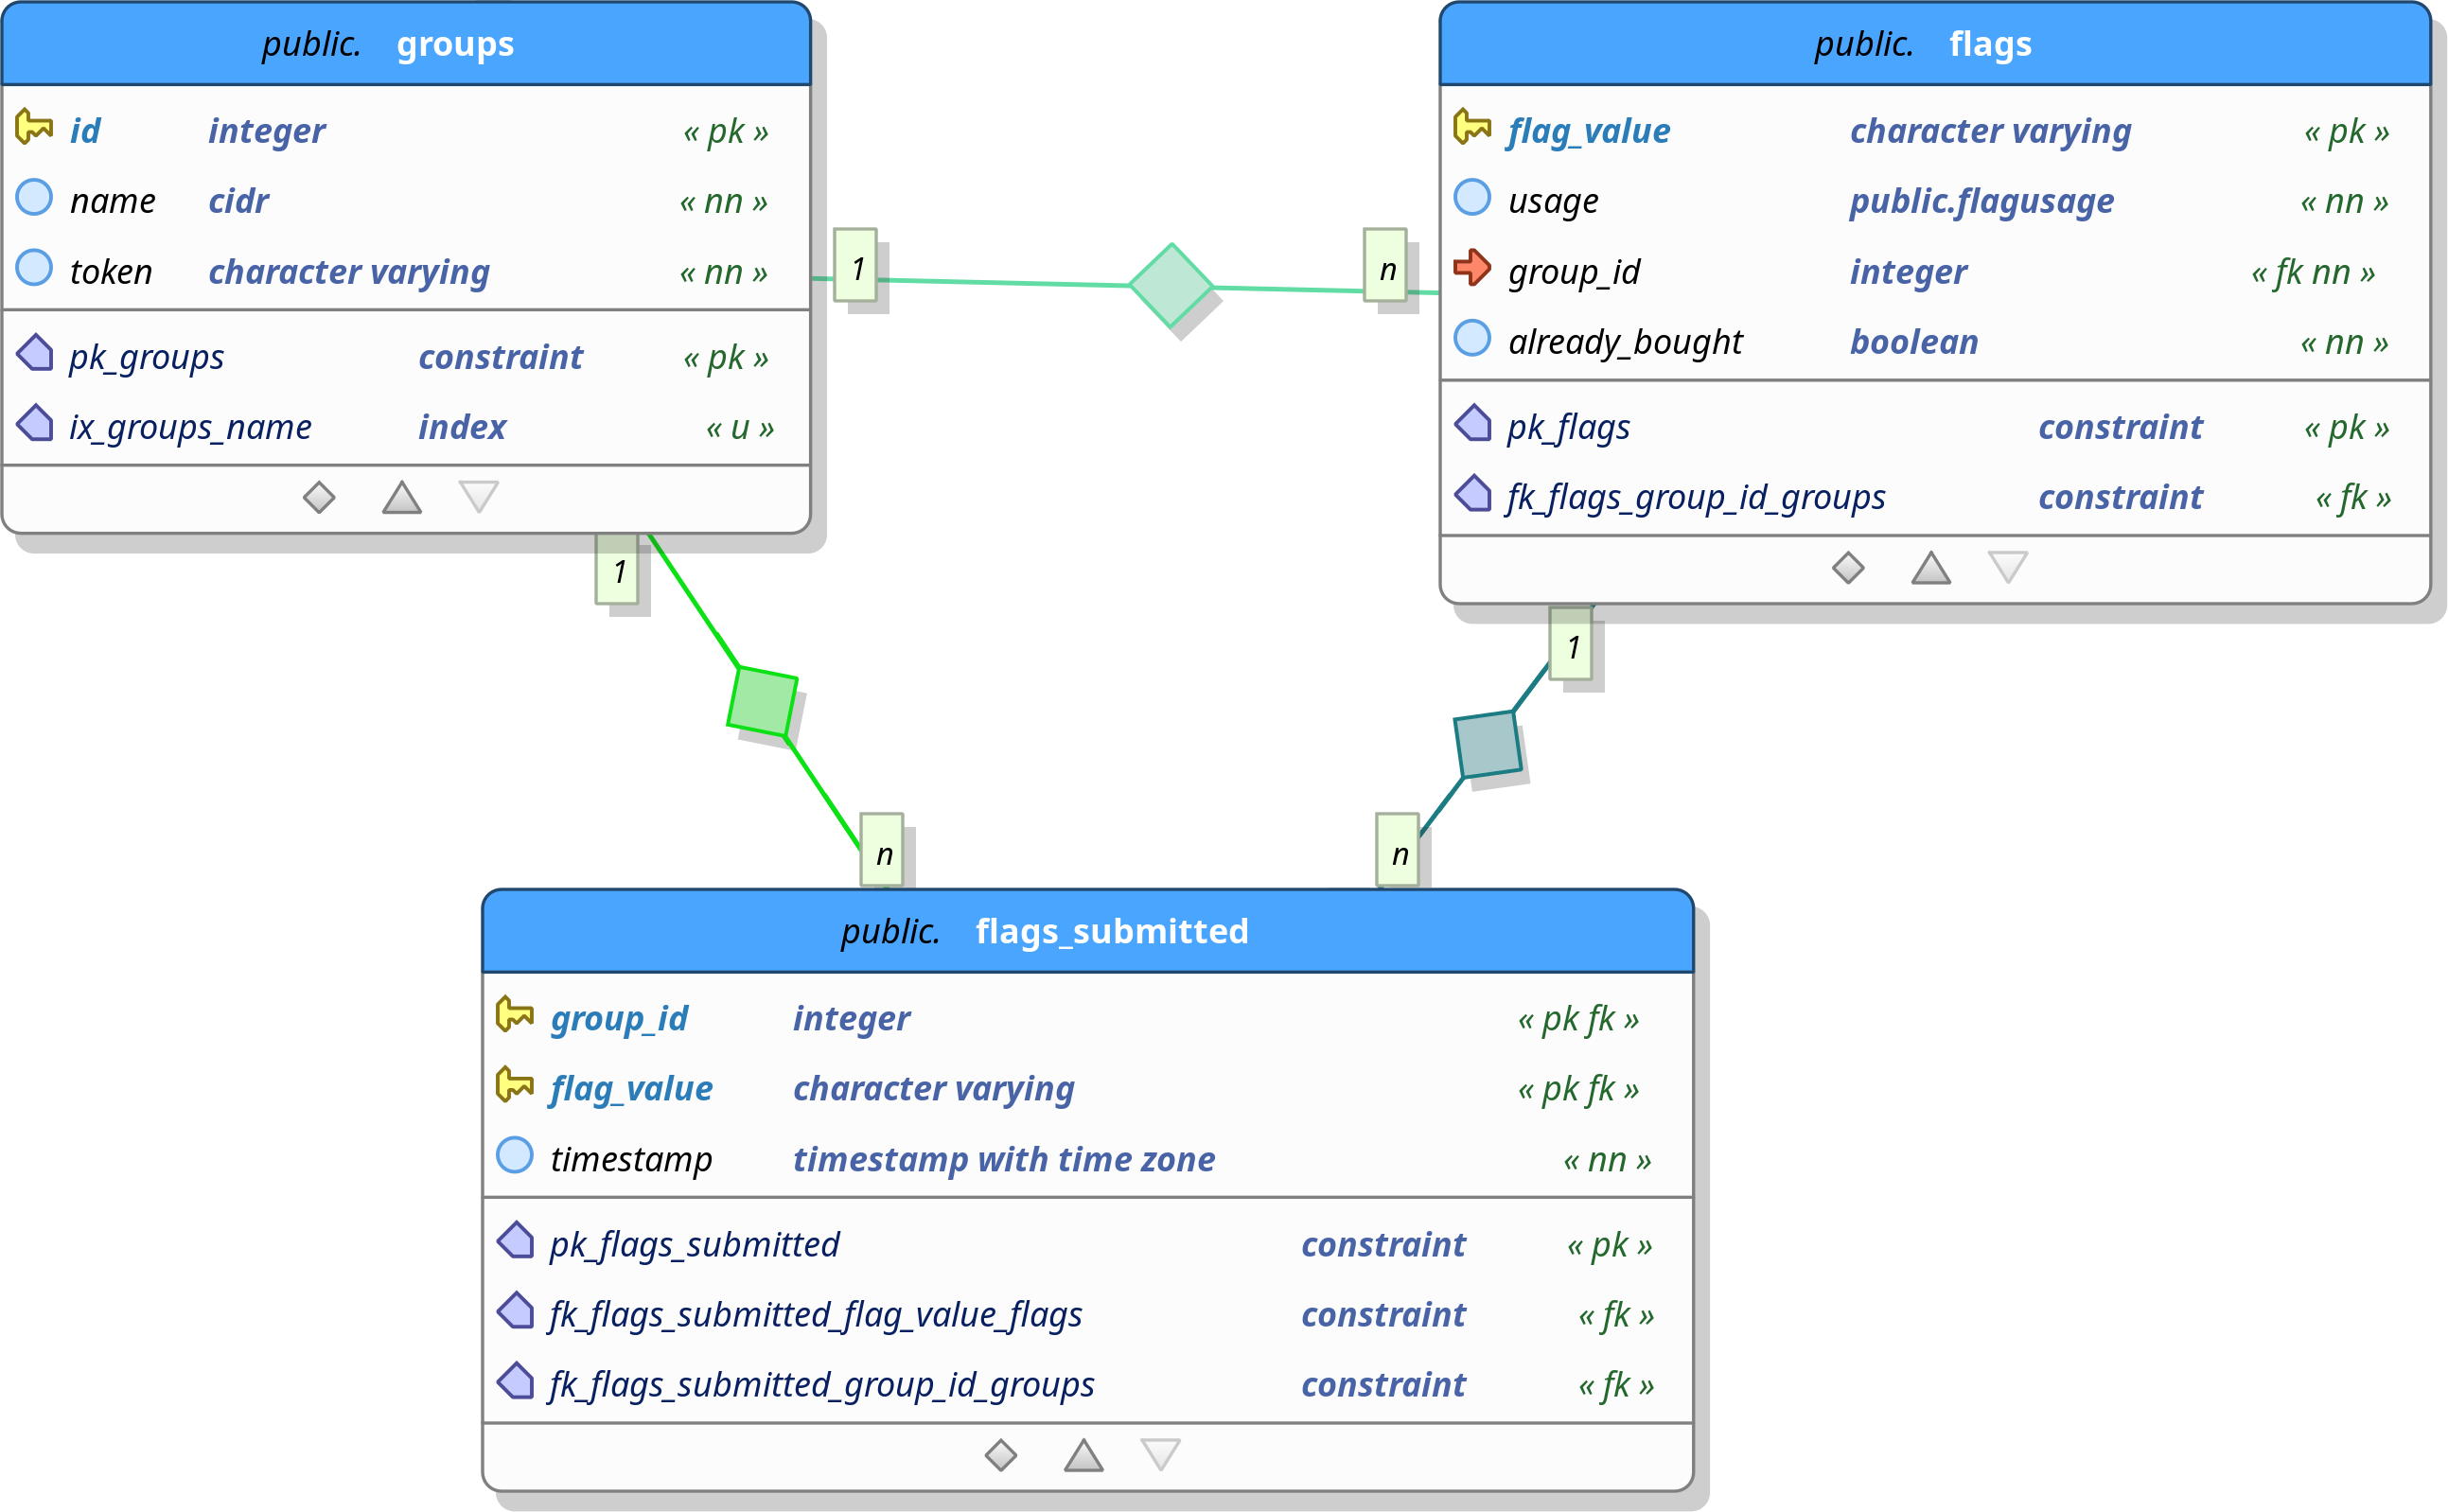
\includegraphics[width=\linewidth, keepaspectratio]{entwurf/datenbank/flags-tabellen}
	\captionof{figure}{Ansicht der Flags-Tabellen (ER-Diagramm)}
	\label{fig:db-flags-table}
\end{center}


In der Abbildung \ref{fig:db-flags-table} erkennbar ist die 1 zu n Beziehung zwischen der Tabelle \textbf{\textit{groups}} und \textbf{\textit{flags}}. Dieses hat zur Folge, dass eine Gruppe mehrere Flags besitzen kann, jedoch eine Flag immer genau zu einer Gruppe gehört. In der Abbildung ist weiter die n zu m Beziehung zwischen \textbf{\textit{groups}} und \textbf{\textit{flags}} abgebildet. Diese wird in eine Verknüpfungstabelle namens \textbf{\textit{flags\_submitted}} mit zwei 1 zu n Beziehung zerlegt. Diese Tabelle enthält die abgegeben Flags.
 
\subsubsection{Flags}
Die während eines Spiels generierten und benötigten Flags werden in der Tabelle \textbf{\textit{flags}} abgelegt. Hierzu wird der Wert der Flag als string in der Spalte \textit{flag\_value} festgehalten. Neben diesem wird Nutzungsart unter Zuhilfenahme eines Enums und die Gruppenzugehörigkeit als Referenz gespeichert. Neben diesem wird in der Spalte \textit{already\_bought} als bool vermerkt, ob diese Flag bereits im Flagshop erworben wurden ist. Diese Spalte besitzt nur Relevanz für die dementsprechenden Flagshop Flags.

\subsubsection{Abgegebene Flags}
Die durch die Studierenden abgegeben Flags werden in der Tabelle \textbf{\textit{flags\_submitted}} eingetragen. Auch wird der Zeitpunkt der Abgabe mitgespeichert, um eventuelle Betrüge aufzudecken. Die Spalten \textit{group\_id} und \textit{flag\_value} bilden zusammen den Primärschlüssel. Dieses ermöglicht, dass jede Gruppe jede Flagge und das eine Gruppe die selbe Flagge nicht mehrfach abgeben kann

\subsection{Service-Tabellen}
\begin{center}
	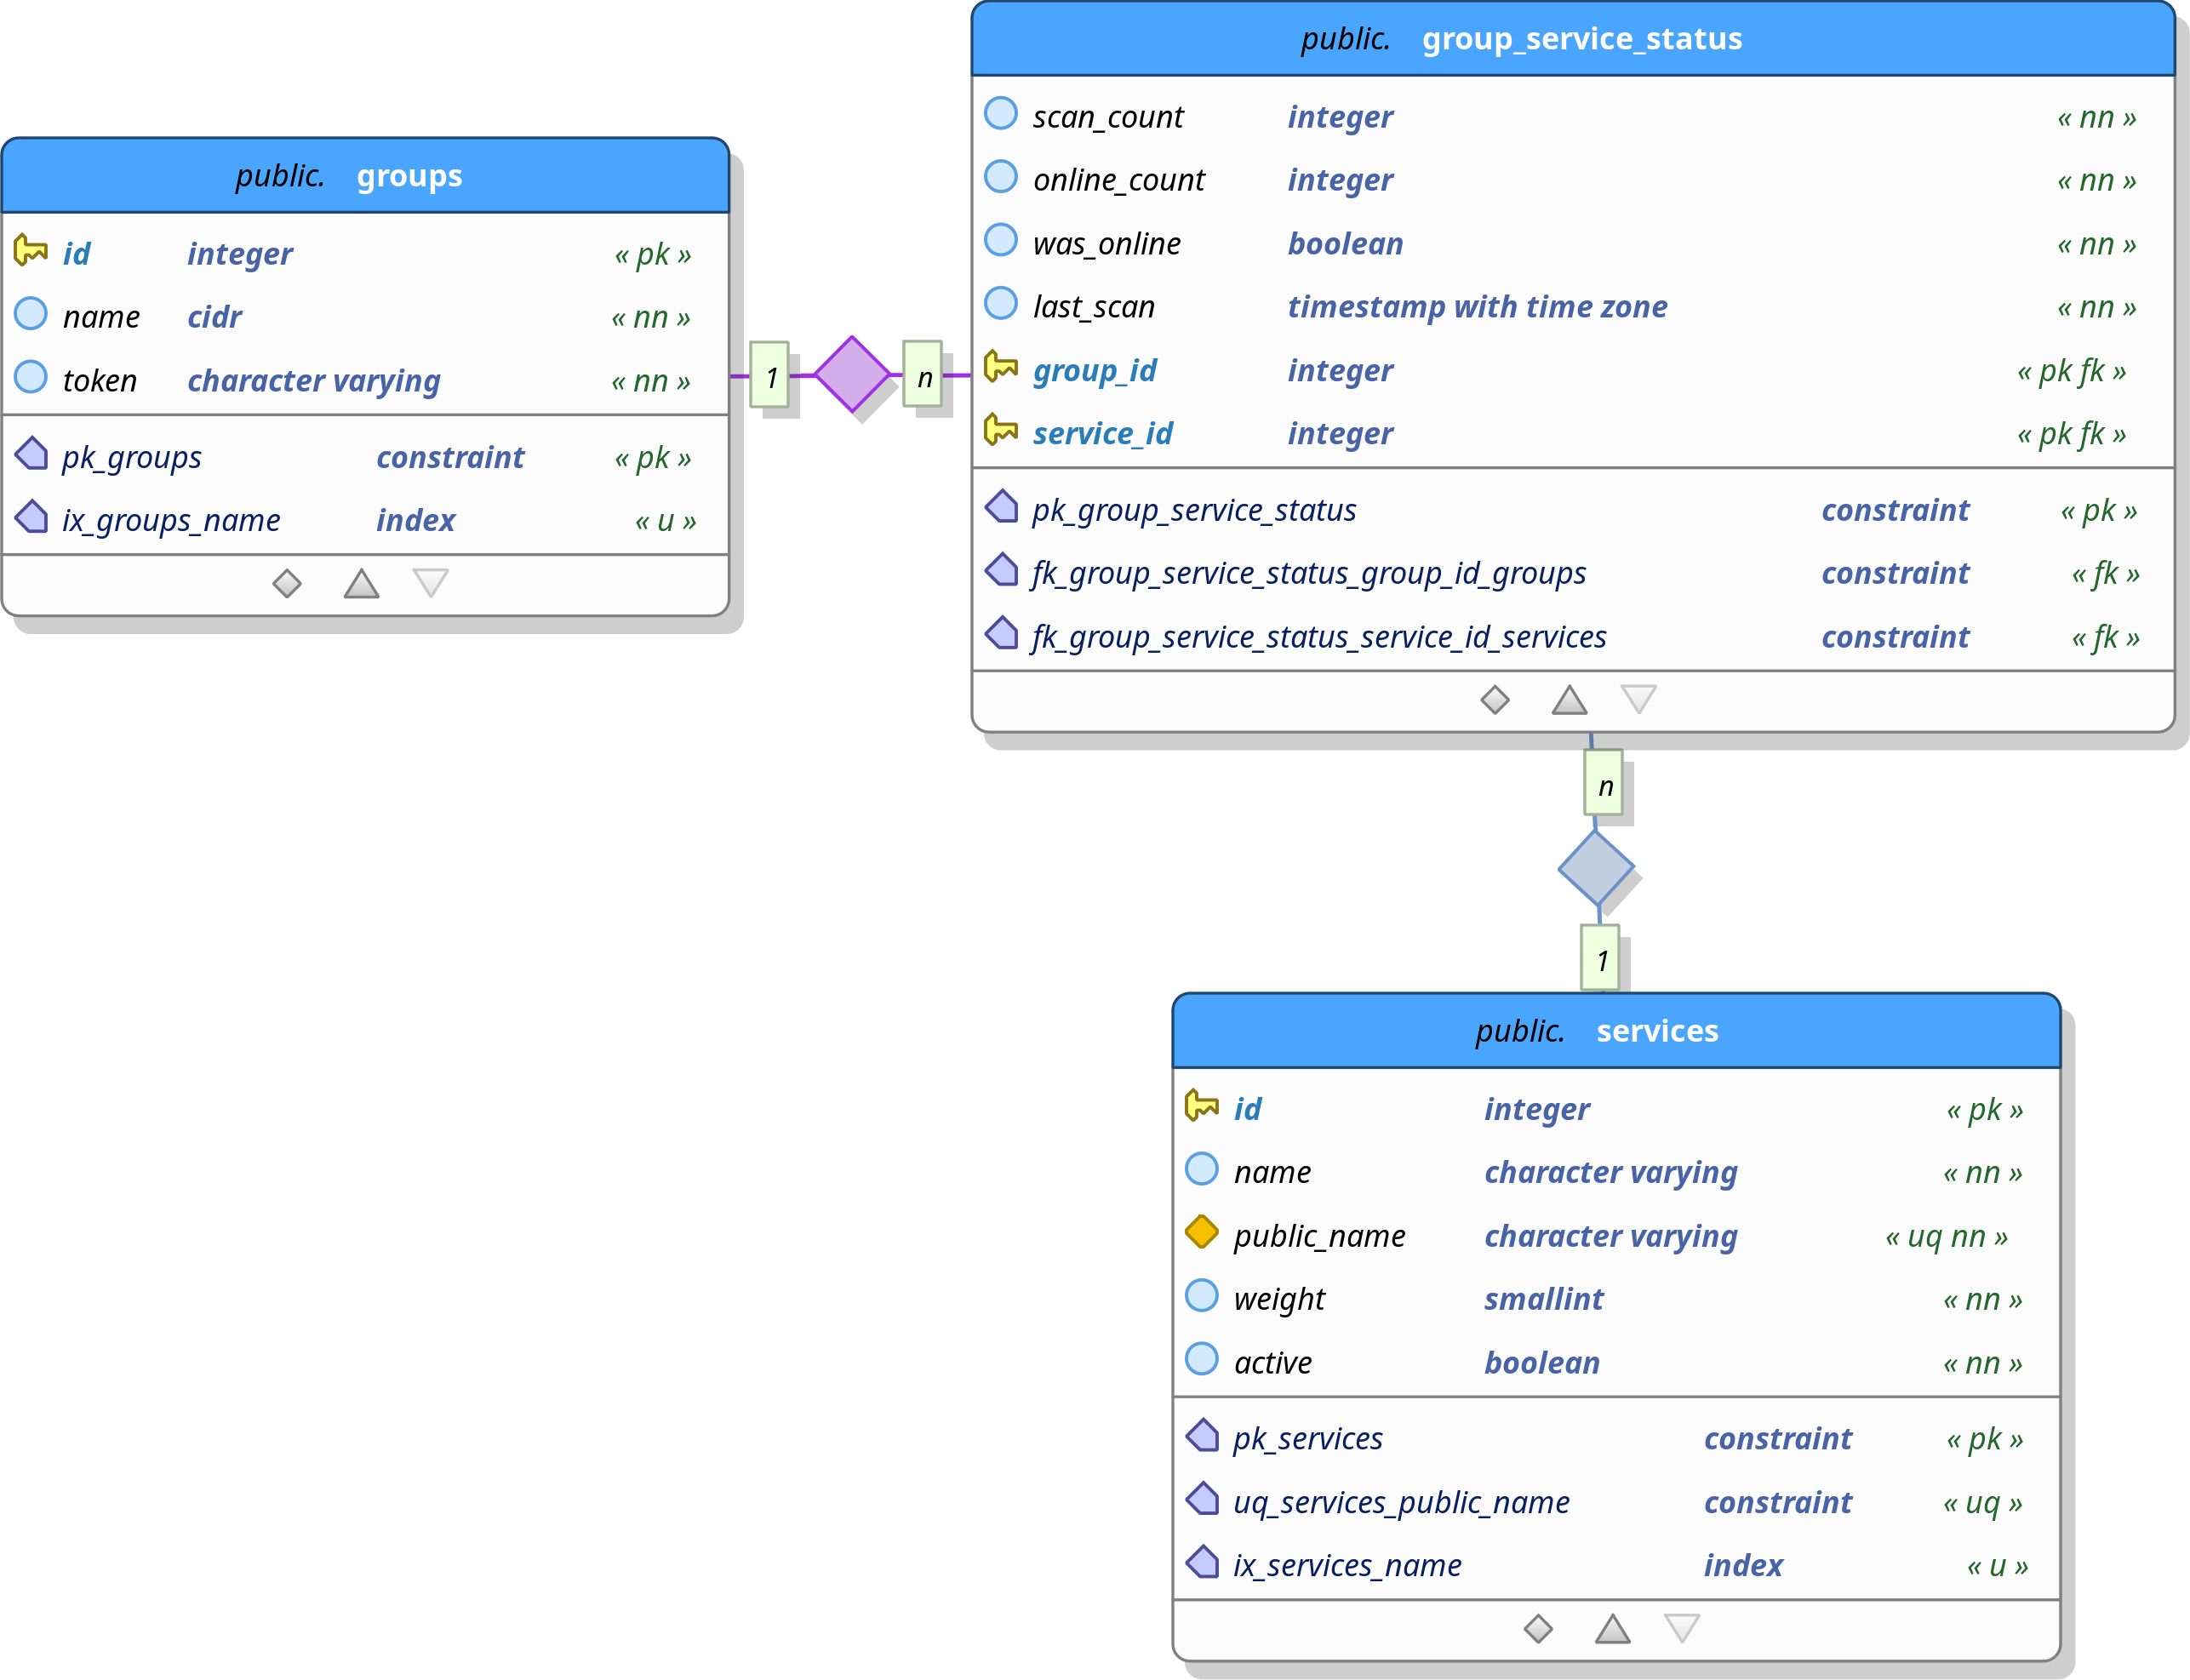
\includegraphics[width=\linewidth, keepaspectratio]{entwurf/datenbank/service-tabellen}
	\captionof{figure}{Ansicht der Service-Tabellen (ER-Diagramm)}
	\label{fig:db-service-table}
\end{center}


In der Abbildung \ref{fig:db-service-table} ist die \textbf{\textit{services}} Tabelle sowie die n zu m Beziehung zwischen \textbf{\textit{groups}} und \textbf{\textit{service}} zu sehen. Diese wird als Referenztabelle (\textbf{\textit{group\_service\_status}}) mit zwei 1 zu n Beziehungen dargestellt.

\subsubsection{Services}
In der \textbf{\textit{services}} Tabelle sind alle vom Big Brother überwachten Schwachstellen eingetragen. Jeder dieser Einträge besteht aus einer eindeutigen ID, dem internen Namen der Operation (\textit{name}), dem angezeigten Namen (\textit{public\_name}) und der Gewichtung des Dienstes im Gesamtergebnis (\textit{weight}). Auch kann die Überprüfung der Schwachstelle mithilfe dem bool-Wert \textit{active} an- oder abgeschaltete werden.

\subsubsection{Servicestatus der Gruppen}
In der Referenztabelle \textbf{\textit{group\_service\_status}} wird das Ergebnis der Überprüfung der Schwachstellen jeder Gruppe abgespeichert. Dazu wird für die Kombination aus Gruppe und Service ein Eintrag angelegt und die Anzahl der Scans in \textit{scan\_count} und die Anzahl der erfolgreichen Scans in \textit{online\_count} gespeichert. Des Weiteren wird der Zeitpunkt des letzten Scans in \textit{last\_scan} und der Erfolg des letzten Scans in \textit{was\_online} festgehalten. Erfolgreich bedeutet in diesem Kontext, dass die Studierenden die überwacht Schwachstelle ausgebessert und den überwachten Dienst online gehalten haben.

\subsection{Flagshop-Tabellen}
\begin{center}
	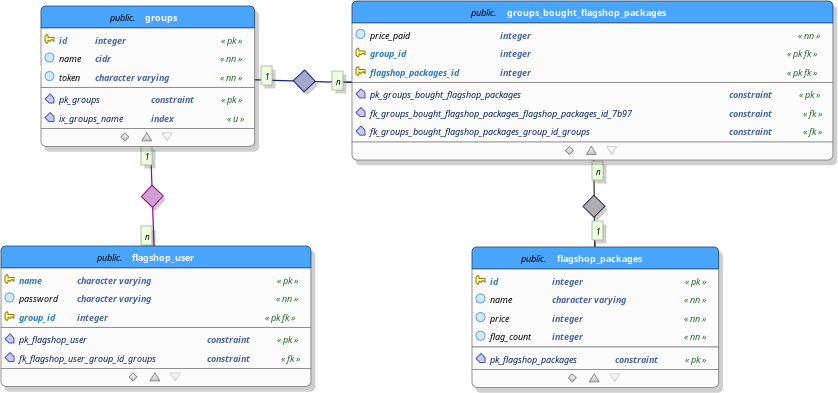
\includegraphics[width=\linewidth, keepaspectratio]{entwurf/datenbank/flagshop-tabellen}
	\captionof{figure}{Ansicht der Flagshop-Tabellen (ER-Diagramm)}
	\label{fig:db-flagshop-table}
\end{center}

Die Abbildung \ref{fig:db-flagshop-table} stellt die 1 zu n Beziehung zwischen den Tabellen \textbf{\textit{groups}} und \textbf{\textit{flagshop\_user}} dar. Das heißt, dass jeder Gruppe mehrere Flagshop Benutzer zugehörig sein können, jeder Benutzer aber genau einer Gruppe angehört. Des Weiteren wird die n zu m Beziehung zwischen \textbf{\textit{groups}} und \textbf{\textit{flagshop\_packages}} als Referenztabelle\\ (\textbf{\textit{groups\_bought\_flagshop\_packages}}) mit zwei 1 zu n Beziehungen dargestellt. Diese beinhaltet die gekauften Flagshop Pakete pro Team.

\subsubsection{Flagshop Nutzer}
Für die Nutzung des Flagshops müssen die Gruppen einen oder mehrere Flagshop Nutzer anlegen. Diese werden in der Tabelle \textbf{\textit{flagshop\_user}} abgelegt. Hierfür wird neben der erstellenden Gruppe (\textit{group\_id}) auch das Passwort (\textit{password}) und der Name (\textit{name})  abgespeichert. Der Primärschlüssel wird aus der Gruppe und dem Namen gebildet. So ist der Nutzername für die Gruppe eindeutig. Mehrere Gruppen können aber Nutzeraccounts mit demselben Namen anlegen.

\subsubsection{Flagshop Pakete}
Die Betreuer und Administratoren können Flagshop Pakete anlegen, welche durch Studierende kaufbar sind. Diese werden in der Tabelle \textbf{\textit{flagshop\_packages}} abgelegt und erhalten Informationen zum Preis (\textit{price}) und der Anzahl der erhaltenen Flags (\textit{flag\_count}). Auch kann ein Name für das Paket über das Feld \textit{name} angegeben werden.

\subsubsection{Gekaufte Flagshop Pakete}
Die durch die Gruppen gekauften Flagshop Pakete werden in der Tabelle\\ \textbf{\textit{group\_bought\_flagshop\_packages}} abgespeichert. Auch wird im Feld \textit{price\_paid} der beim Kauf gezahlte Preis festgehalten, da die Studierenden den Preis eines Flagshop Paketes beim Kauf reduzieren können. Jedes Paket kann genau einmal von jeder Gruppe gekauft werden, da sich der Primärschlüssel aus Gruppe (\textit{group\_id}) und Paket (\textit{flagshop\_packages\_id}) zusammen setzt.

\subsection{Challenge-Tabellen}
\begin{center}
	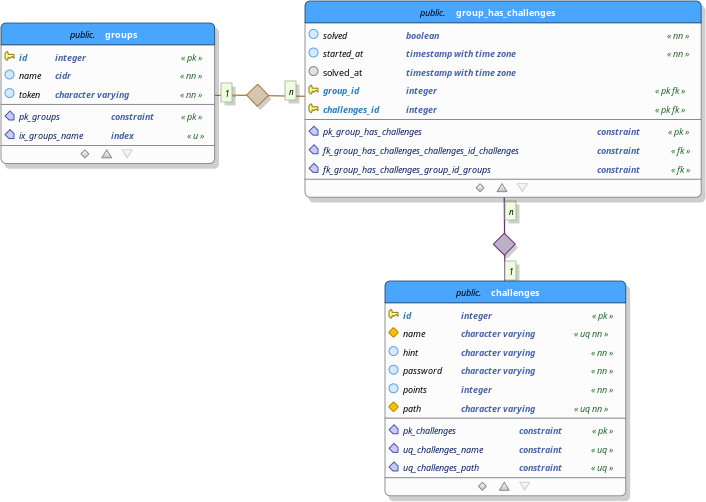
\includegraphics[width=\linewidth, keepaspectratio]{entwurf/datenbank/challenge-tabellen}
	\captionof{figure}{Ansicht der Service-Tabellen (ER-Diagramm)}
	\label{fig:db-challenge-table}
\end{center}
In der Abbildung \ref{fig:db-challenge-table} ist die \textbf{\textit{Challenge}} Tabelle und die n zum m Beziehung zwischen den Tabelle \textbf{\textit{groups}} und \textbf{\textit{challenges}} zusehen. Diese Beziehung ist als Verknüpfungstabelle (\textbf{\textit{group\_has\_challenges}}) mit zwei 1 zu n Beziehung realisiert.

\subsubsection{Challenges}
Die \textbf{\textit{challenges}} Tabelle beinhaltet alle Challenges, welche von den Studierenden gelöst werden können. Jede Challenge besitzt eine eindeutige ID. Neben dieser wird für jede Challenge ein Titel / Name in \textit{name}, ein Hinweis in \textit{hint}, das zum Lösen benötigte Passwort in \textit{password}, die Anzahl der Punkte in \textit{points} und der Pfad, über den die Challenge abgerufen werden kann, gespeichert.

\subsubsection{Gestartete / Abgeschlossene Challenges}
Alle angefangen und abgeschlossenen Challenges werden in der Tabelle \textbf{\textit{group\_has\_challenges}} abgespeichert. Es wird das Startdatum (\textit{started\_at}) der Challenge, den Status des Abschluss (\textit{solved}) und bei erfolgreicher Absolvierung der Challenge das Enddatum ((\textit{solved\_at})) gespeichert. Durch die Zusammensetzung des Primärschlüssel aus Challenge und Gruppe, kann jede Gruppe jede Challenge genau einmal starten und absolvieren.

\subsection{Weitere Tabellen}
\begin{center}
	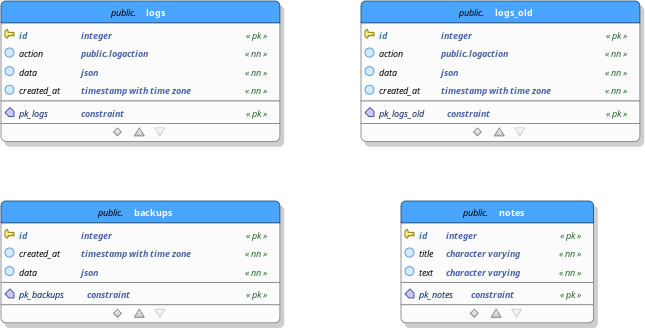
\includegraphics[width=\linewidth, keepaspectratio]{entwurf/datenbank/etc-tabellen}
	\captionof{figure}{Ansicht der weiteren Tabellen (ER-Diagramm)}
	\label{fig:db-etc-table}
\end{center}

Wie in Abbildung \ref{fig:db-etc-table} erkennbar besitzen die Tabellen keine Abhängigkeiten und Verbindungen zu anderen. Im Folgenden werden die Tabellen für die Logs, die Notizen und die alten Spielstände vorgestellt.

\subsubsection{Logs}
Um die Aktionen innerhalb der Anwendung nachverfolgen zu können, werden diese in die \textbf{\textit{logs}} Tabelle geschrieben. Jeder Eintrag besteht aus einer ID, einem Enum in dem der Typ der Aktion festgehalten wird (\textit{action}), einem Zeitpunkt (\textit{timestamp}) und dem Inhalt der Aktion \textit{data}. 

Innerhalb der \textbf{\textit{logs}} Tabelle werden nur die Aktionen des derzeitig aktiven Spiels gespeichert. Neben diesen werden auch noch die Aktionen des letzten Spiels in der Tabelle \textbf{\textit{logs\_old}} gespeichert. Sollte ein Spiel beendet werden, werden die Aktionen des alten Spiels mit den neuen Aktionen überschrieben.

\subsubsection{Notizen}
In der Tabelle \textbf{\textit{notes}} soll den Betreuern und Administratoren die Möglichkeit geboten werden Notizen und Hinweise zum Rahmen und Durchführung des Versuches zu geben. Diese Notizen können durch die Studierenden eingesehen werden. Dafür werden Titel und Inhalt jeweils in einem string gespeichert. Um einzelne Notizen abrufen zu können, erhalten diese eine eindeutige ID.

\subsubsection{Alte Spiele}
Die Tabelle \textbf{\textit{backups}} soll alle alten Spielstände speichern. Dazu wird jedem Backup eine eindeutige ID zugewiesen und der Zeitpunkt des Erstellens wird in \textit{created\_at} abgespeichert. Die Informationen zu einem Spiel sind im JSON Format in der Spalte \textit{data} abgelegt.